\newpage
\section{Analyse du besoin et étude préalable}

Ce chapitre présente le contexte général du projet CYBEL ainsi que l'analyse
du besoin ayant conduit à la définition de la solution proposée. Il met en
évidence l'architecture du système étudié, la problématique associée, les
objectifs du projet ainsi que le cahier des charges fonctionnel et technique.

\subsection{Contexte du projet}

\subsubsection*{Présentation du robot CIOT TY1251D-03195}

Le robot étudié est un \textbf{robot de réception mobile} commercialisé sous la
référence \textbf{CIOT TY1251D-03195} illustré sur la  figure~\ref{fig:robot}. Il est composé de deux sous-systèmes
matériels distincts, reliés en interne :

\begin{itemize}
    \item un \textbf{châssis de navigation} fonctionnant sous \textbf{Linux
    embarqué avec ROS}, responsable de la localisation (SLAM), de la planification
    de trajectoire (\texttt{move\_base}) et de l'exécution des commandes de
    mouvement ;
    \item un \textbf{\og upper body \fg{} Android 7.1} (SoC RK3399, 2 Go de RAM,
    16 Go de stockage), équipé d'un écran tactile 15,6" (1920×1080), de caméras
    (reconnaissance faciale, surveillance) et de haut-parleurs, qui héberge
    l'application propriétaire d'accueil et l'interface utilisateur standard du
    robot.
\end{itemize}

Le robot dispose d'un point d'accès WiFi propre (\texttt{TY1251D-03195})
permettant à un poste externe de rejoindre son réseau local. La topologie
réseau s'est révélée plus complexe que ne le laissait supposer une simple
architecture à deux hôtes : le châssis est joignable à l'adresse fixe
\texttt{10.42.0.1}, tandis que la tête Android obtient une adresse variable
par DHCP sur un second segment \texttt{172.16.0.0/16} une première IP
documentée (\texttt{172.16.0.88}) s'est révélée périmée en cours de projet.
Les deux sous-systèmes sont par ailleurs reliés en interne par une liaison
filaire \texttt{eth0} sur le segment \texttt{192.168.20.0/24}
(\texttt{192.168.20.1} pour la tête, \texttt{192.168.20.22} pour le châssis),
indépendante du réseau WiFi exposé à l'extérieur.

\begin{center}
    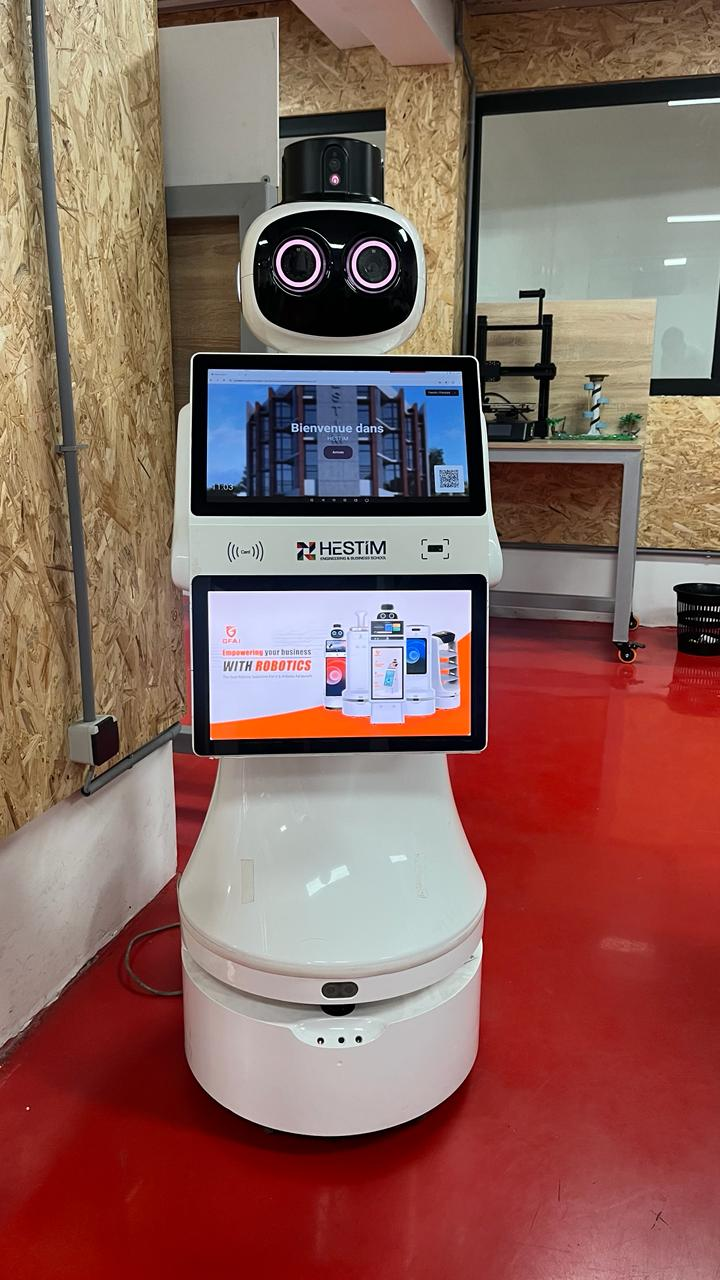
\includegraphics[width=0.4\textwidth]{images/cybel.jpeg}
    \captionof{figure}{Robot CIOT TY1251D-03195 "CYBEL"}
    \label{fig:robot}
\end{center}

\subsubsection*{Architecture générale du robot}

Vue dans son ensemble, l'architecture du système peut se lire en quatre
couches superposées, illustrées en figure~\ref{fig:archi_robot} : une couche
de présentation et d'interaction, une couche applicative et API, une couche
de communication et de services réseau, et une couche matérielle.

\paragraph{Couche de présentation et d'interaction (couche supérieure):}Au sommet de l'architecture se trouve la couche de présentation, qui regroupe
l'ensemble des interfaces utilisateur permettant d'interagir avec le robot.
On y distingue trois composants principaux : l'\textbf{application
propriétaire Android}, considérée comme une boîte noire non documentée et
hors du périmètre du projet ; l'\textbf{interface opérateur web (CYBEL)},
développée dans le cadre du projet et permettant le contrôle et la
supervision du robot ; et l'\textbf{interface visiteur (mode kiosque)},
dédiée aux interactions simplifiées dans un contexte public. Cette couche
constitue le point d'entrée principal des interactions homme-machine et
repose sur des échanges réseau vers les couches inférieures, notamment via
HTTP et WebSocket. Deux composants complémentaires y sont également présents
côté Android : un module de \textbf{synthèse vocale (TTS natif)}, permettant
les retours audio du robot, et un mode \textbf{WebView kiosque}, utilisé pour
des interactions simplifiées embarquées.

\paragraph{Couche applicative et API (couche intermédiaire):}
La deuxième couche correspond à la logique applicative centrale du système,
matérialisée par l'\textbf{API CYBEL développée en FastAPI}. Cette API joue
un rôle d'orchestrateur entre les interfaces utilisateur et les mécanismes
de communication avec le robot : elle expose des endpoints REST ainsi que
des canaux WebSocket pour la supervision en temps réel. Elle est alimentée
par deux types de clients un \textbf{SDK Python en mode réel}, qui assure
la communication directe avec le robot, et un \textbf{SDK Python en mode
simulé (\textit{mock})}, permettant le développement et les tests
indépendamment du matériel. Ces deux modes convergent vers une interface
commune abstraite (\texttt{RobotBackend}), garantissant la continuité
fonctionnelle entre simulation et exécution réelle.

\paragraph{Couche de communication et de services réseau:}
La troisième couche représente les interfaces réseau exposées par le robot
et utilisées comme points d'accès aux fonctionnalités internes. Elle
comprend plusieurs services distincts : \textbf{rosbridge} (WebSocket, port
9090), permettant l'envoi et la réception de messages ROS au format JSON ;
\textbf{rosapi}, utilisé pour l'introspection des topics, services et
abonnés ROS ; \textbf{MQTT} (port 1883), employé pour la communication
événementielle et la télémétrie ; et \textbf{ADB} (\textit{Android Debug
Bridge}), offrant un accès direct au sous-système Android. Cette couche
constitue le point d'interconnexion critique entre la logique applicative
CYBEL et le système robotique réel.

\paragraph{Couche matérielle et système robotique:}
À la base de l'architecture se trouve la couche matérielle, composée des
deux sous-systèmes principaux du robot. D'une part, le \textbf{châssis de
navigation} sous Linux embarqué avec ROS assure les fonctions de mobilité :
il intègre les modules de SLAM, de planification de trajectoire
(\texttt{move\_base}) et les capteurs de perception tels que le LiDAR, et
reste accessible via l'adresse réseau interne \texttt{10.42.0.1}. D'autre
part, le \textbf{module supérieur Android} constitue la partie interactive
du robot : il regroupe l'écran tactile, les caméras, les haut-parleurs et
les applications utilisateur, et reste accessible via un réseau interne
distinct (\texttt{172.16.0.0/16}). Ces deux sous-systèmes communiquent entre
eux via la liaison Ethernet interne décrite plus haut, assurant la
synchronisation entre navigation et interaction utilisateur.

\begin{center}
    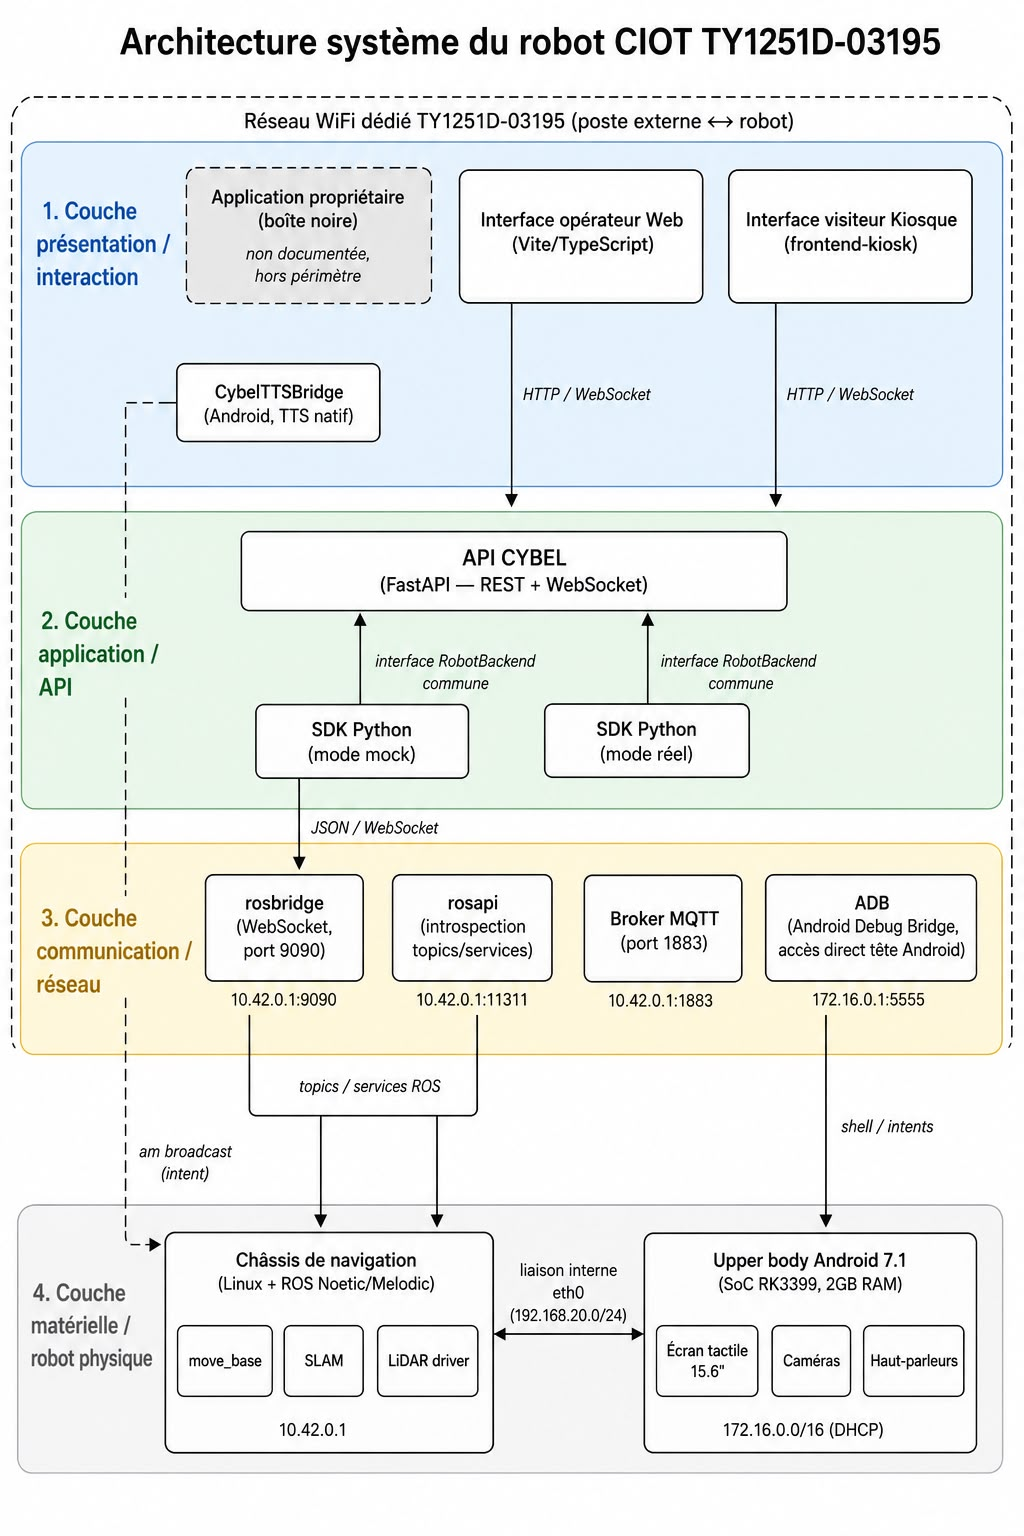
\includegraphics[width=0.7\textwidth]{diagramme/architecture_globale.jpeg}
    \captionof{figure}{Architecture système globale du robot CIOT TY1251D-03195}
    \label{fig:archi_robot}
\end{center}

\paragraph{Positionnement du système CYBEL dans l'architecture.}
Le système CYBEL s'insère principalement dans les couches supérieures de
l'architecture, en remplaçant et en étendant les capacités de l'application
propriétaire. Il s'appuie sur la couche applicative (API FastAPI et SDK
Python) pour structurer la logique de commande, sur la couche réseau
(rosbridge, MQTT) pour l'interaction avec le robot, et sur les couches
matérielles sous-jacentes pour l'exécution des actions physiques. Cette
approche permet de découpler totalement l'interface utilisateur du système
robotique, tout en garantissant une compatibilité avec l'infrastructure
existante.

L'architecture globale du système met ainsi en évidence une organisation en
couches clairement séparées, allant de l'interface utilisateur jusqu'au
matériel robotique. Cette structuration constitue le fondement de la
solution CYBEL, qui s'inscrit comme une couche logicielle intermédiaire
visant à unifier, simplifier et étendre l'accès aux fonctionnalités du robot
CIOT TY1251D-03195.

\subsubsection*{Cadre et déroulement du stage}

L'établissement disposant de ce robot souhaite l'utiliser pour des scénarios
d'accueil et de démonstration personnalisés : annonces vocales spécifiques,
déplacements vers des points définis par l'utilisateur, supervision à
distance. Le projet est encadré par HESTIM Engineering \& Business School et
s'adresse à des étudiants du cycle ingénieur (dont la
1\textsuperscript{re} année). Il est prévu sur une durée de trois à quatre mois, structuré en
quatre phases : (1) compréhension de l'architecture et établissement de la
connectivité réseau, (2) exploration et analyse du protocole de
communication interne, (3) développement de l'interface de commande et des
modules d'interaction, et (4) intégration, tests et validation finale.

\subsubsection*{Limites de la solution existante}

L'application propriétaire installée sur l'\textit{upper body} ne permet pas
le type de personnalisation recherché : elle constitue une boîte noire, sans
documentation, sans API exposée et sans code source disponible. Le
constructeur ne fournit par ailleurs aucune documentation technique sur les
protocoles de communication internes, ce qui interdit toute extension ou
adaptation directe de la solution d'origine.

\subsection{Problématique}

La problématique centrale du projet peut être formulée ainsi :

\begin{center}
\fbox{
    \parbox{0.9\textwidth}{
        \textit{Comment concevoir une plateforme de commande et d'interaction
        tierce, fonctionnellement équivalente ou supérieure à l'application
        propriétaire d'un robot de service Android, en l'absence de toute
        documentation officielle sur ses interfaces de communication internes ?}
    }
}
\end{center}

\medskip
Cette problématique se décline en plusieurs sous-questions :

\begin{itemize}
    \item Quels sont les \textbf{points d'accès réseau} (adresses IP, ports,
    protocoles) exposés par le robot, et lesquels sont effectivement exploitables
    sans authentification propriétaire ?
    \item Quel est le \textbf{format des messages} échangés entre l'interface
    Android et le système de navigation (ROS), et peut-il être reconstruit par
    observation et introspection plutôt que par décompilation de l'application ?
    \item Comment \textbf{distinguer une commande effectivement traitée par le
    robot d'une commande silencieusement ignorée}, dans un système où le protocole
    de transport (\texttt{rosbridge}) ne renvoie pas systématiquement d'erreur
    explicite ?
    \item Comment concevoir une architecture logicielle qui reste
    \textbf{utilisable et testable sans accès permanent au robot physique}
    (contraintes de disponibilité du matériel), tout en restant fidèle au
    comportement réel une fois connectée ?
    \item Dans quelle mesure les fonctionnalités d'\textbf{interaction homme-robot}
    (synthèse vocale, reconnaissance vocale, retour visuel) peuvent-elles être
    reconstruites lorsque le canal correspondant n'est pas exposé par le système
    de navigation (ROS) et nécessite un accès direct au sous-système Android ?
\end{itemize}

\subsection{Objectifs du projet}

\subsubsection{Objectif général}

Concevoir et développer une \textbf{plateforme web indépendante} de commande,
de supervision et d'interaction pour le robot CIOT TY1251D-03195, sans
dépendre de l'application Android propriétaire, en documentant de façon
rigoureuse le \textbf{protocole de communication} reconstruit (endpoints,
topics, services, formats de messages) afin que ce travail puisse être
réutilisé ou étendu.

\subsubsection{Objectifs spécifiques}

\begin{enumerate}
    \item \textbf{Établir la connectivité} avec le robot (réseau WiFi dédié,
    identification des hôtes et ports actifs).
    \item \textbf{Identifier les points de communication} exposés : WebSocket
    \texttt{rosbridge} (port 9090), broker \texttt{MQTT} (port 1883), services
    FTP/SSH, interfaces web internes (\texttt{:8082}, \texttt{:8088}).
    \item \textbf{Capturer et analyser le trafic réseau} afin de reconstituer
    les topics et services ROS pertinents (mouvement, navigation, télémétrie,
    capteurs).
    \item \textbf{Décoder et reconstruire les commandes de contrôle} du
    mouvement et de la navigation (vitesse, position cible, annulation de
    trajectoire).
    \item \textbf{Développer une interface de commande web} (backend FastAPI
    + frontend TypeScript) permettant la supervision temps réel et l'envoi de
    commandes.
    \item \textbf{Implémenter des fonctionnalités d'interaction homme-robot de
    base} : navigation par sélection de points ou clic sur carte, retour vocal
    (TTS) et commande vocale opérateur.
    \item \textbf{Mettre en place un mode de simulation (« mock »)} permettant
    de développer et tester l'interface sans dépendre de la disponibilité
    physique du robot.
    \item \textbf{Intégrer l'ensemble des composants} (SDK Python, API, interface
    web) dans un système cohérent et démontrable.
\end{enumerate}

\subsection{Cahier des charges}

\subsubsection{Périmètre du projet}

Le tableau~\ref{tab:perimetre_projet} délimite les activités prises en
charge par le projet de celles volontairement laissées hors périmètre.

\begin{center}
\begin{tabular}{|p{0.46\textwidth}|p{0.46\textwidth}|}
\hline
\textbf{Inclus dans le périmètre} & \textbf{Exclu du périmètre} \\
\hline
Identification et documentation des canaux de communication du robot
(\texttt{rosbridge}, MQTT, services réseau) &
Modification du firmware ou du logiciel embarqué du robot \\
\hline
Développement d'un SDK Python d'accès au robot (mode simulé et mode réel) &
Développement d'une application Android de remplacement (optionnel, non engagé) \\
\hline
Développement d'une API de commande/supervision (FastAPI) &
Décompilation ou rétro-ingénierie de l'application Android propriétaire \\
\hline
Développement d'une interface web opérateur (Vite/TypeScript) &
Déploiement en production / hébergement distant \\
\hline
Fonctionnalités de navigation (point nommé, clic sur carte, téléopération) &
Comportements autonomes avancés (planification de mission, multi-robot) \\
\hline
Interaction de base : synthèse vocale (TTS) et commande vocale opérateur &
Vision par caméra, reconnaissance faciale, chatbot (extensions optionnelles) \\
\hline
Documentation technique et rapport de stage &
Formation des utilisateurs finaux / exploitation au long cours \\
\hline
\end{tabular}
\captionof{table}{Périmètre du projet : éléments inclus et exclus}
\label{tab:perimetre_projet}
\end{center}

\subsubsection{Acteurs du système}

Le tableau~\ref{tab:acteurs_systeme} identifie les principaux acteurs
impliqués dans le projet ainsi que leur rôle respectif.

\begin{center}
\begin{tabular}{|p{0.35\textwidth}|p{0.57\textwidth}|}
\hline
\textbf{Acteur} & \textbf{Rôle} \\
\hline
Étudiant(e) stagiaire — plateforme CYBEL (C. Lusamote Kimfuta) &
Rétro-ingénierie, SDK, backend, interfaces web, Android, déploiement Termux,
documentation technique, contenu du présent rapport \\
\hline
Étudiant(e) stagiaire — chatbot (G. Khalifi) &
Développement d'un module chatbot sur la branche
\texttt{chatbot-cybel-projet-2026} du dépôt GitHub (hors périmètre CYBEL) \\
\hline
Encadrante pédagogique (Mme MESKINI, HESTIM) &
Suivi pédagogique, validation académique du rapport \\
\hline
Encadrant en entreprise (M. Tula, HESTIM) &
Suivi technique du robot, validation des objectifs sur le terrain \\
\hline
Établissement d'accueil &
Mise à disposition du robot et de l'environnement de travail \\
\hline
Opérateur final &
Supervision et pilotage du robot via la plateforme CYBEL \\
\hline
Robot CIOT TY1251D-03195 &
Système cible — serveur de télémétrie et de commandes via \texttt{rosbridge}/MQTT \\
\hline
\end{tabular}
\captionof{table}{Acteurs du système et leurs rôles}
\label{tab:acteurs_systeme}
\end{center}

\subsubsection{Besoins fonctionnels}

Le tableau~\ref{tab:besoins_fonctionnels} liste les exigences fonctionnelles
du système, accompagnées de leur niveau de priorité.

\begin{center}
\begin{tabular}{|p{0.10\textwidth}|p{0.67\textwidth}|p{0.13\textwidth}|}
\hline
\textbf{Réf.} & \textbf{Exigence} & \textbf{Priorité} \\
\hline
EF-01 & Superviser en temps réel l'état du robot (batterie, position, statut,
mode de navigation) & Essentielle \\
\hline
EF-02 & Afficher la carte SLAM, le LiDAR et les personnes détectées & Essentielle \\
\hline
EF-03 & Naviguer vers un point nommé prédéfini & Essentielle \\
\hline
EF-04 & Naviguer vers une coordonnée choisie par clic sur la carte, avec prise
en compte des obstacles & Essentielle \\
\hline
EF-05 & Téléopérer manuellement le robot (vitesse linéaire/angulaire) avec arrêt
d'urgence & Essentielle \\
\hline
EF-06 & Déclencher une annonce vocale sur le robot (TTS) & Souhaitable \\
\hline
EF-07 & Donner des commandes vocales à l'opérateur via le micro du navigateur &
Souhaitable \\
\hline
EF-08 & Configurer les paramètres de fonctionnement (vitesse, mode de
déplacement) & Souhaitable \\
\hline
EF-09 & Fonctionner en mode simulation complet sans robot connecté & Essentielle \\
\hline
\end{tabular}
\captionof{table}{Besoins fonctionnels du système}
\label{tab:besoins_fonctionnels}
\end{center}

\subsubsection{Besoins non fonctionnels}

Le tableau~\ref{tab:besoins_non_fonctionnels} présente les exigences non
fonctionnelles, relatives notamment à la performance, à la robustesse et à
la séparation des responsabilités au sein de l'architecture.

\begin{center}
\begin{tabular}{|p{0.10\textwidth}|p{0.67\textwidth}|p{0.13\textwidth}|}
\hline
\textbf{Réf.} & \textbf{Exigence} & \textbf{Priorité} \\
\hline
ENF-01 & Latence d'affichage de la télémétrie de l'ordre de quelques centaines
de ms maximum & Essentielle \\
\hline
ENF-02 & Reconnexion automatique au robot après perte de connexion réseau &
Essentielle \\
\hline
ENF-03 & Séparation stricte entre couche d'accès robot (SDK), API et présentation
& Essentielle \\
\hline
ENF-04 & Toute commande de mouvement/navigation doit être annulable à tout moment
& Essentielle \\
\hline
ENF-05 & Aucune action exploratoire ne doit perturber le fonctionnement normal
du robot & Essentielle \\
\hline
\end{tabular}
\captionof{table}{Besoins non fonctionnels du système}
\label{tab:besoins_non_fonctionnels}
\end{center}

\subsubsection{Contraintes du projet}

\begin{itemize}
    \item \textbf{Contraintes techniques} : absence de documentation officielle
    du protocole ; dépendance à un réseau WiFi dédié et potentiellement instable
    (latence variable, de 7 à 1654 ms observés) ; version Android embarquée
    obsolète (7.1) limitant les outils de débogage disponibles.

    \item \textbf{Contraintes matérielles} : un seul exemplaire de robot
    disponible, partagé avec d'autres usages de l'établissement — disponibilité
    limitée pour les tests.

    \item \textbf{Contraintes organisationnelles} : durée de stage limitée à
    trois à quatre mois ; deux stagiaires avec des périmètres distincts
    (plateforme CYBEL et chatbot) ; encadrement pédagogique et terrain
    périodique.

    \item \textbf{Contraintes de sécurité et d'éthique} : les canaux
    \texttt{rosbridge} et MQTT du robot étant accessibles sans authentification,
    toute manipulation doit respecter un principe de \textbf{précaution}
    (vérification en mode simulation avant toute commande réelle, mécanisme
    d'annulation disponible) ; les tentatives d'accès aux comptes système (SSH/FTP)
    doivent rester mesurées pour ne pas provoquer de blocage.

    \item \textbf{Contraintes de propriété intellectuelle} : aucune décompilation
    du logiciel propriétaire n'est entreprise ; seule l'observation du trafic
    réseau et l'introspection des interfaces standard (ROS, MQTT) sont utilisées.
\end{itemize}

\subsubsection{Livrables attendus}

Conformément au sujet de stage, les livrables attendus en fin de projet sont :

\begin{enumerate}
    \item Une \textbf{interface de communication fonctionnelle} avec le robot
    (SDK + client \texttt{rosbridge}/MQTT).
    \item Un \textbf{système de contrôle du mouvement} opérationnel
    (téléopération + navigation).
    \item Une \textbf{interface utilisateur} web opérateur.
    \item Un \textbf{module d'interaction de base} (tactile et/ou vocal).
    \item Un \textbf{rapport technique} incluant l'architecture du système et
    l'analyse du protocole.
\end{enumerate}

\subsubsection{Critères de réception et de validation}

Le tableau~\ref{tab:criteres_validation} précise, pour chaque critère
d'acceptation, la modalité de vérification associée.

\begin{center}
\begin{tabular}{|p{0.40\textwidth}|p{0.52\textwidth}|}
\hline
\textbf{Critère} & \textbf{Modalité de vérification} \\
\hline
Connexion au robot établie de façon reproductible &
Connexion \texttt{rosbridge} réussie depuis le réseau WiFi du robot, vérifiable
via \texttt{/rosapi/topics} \\
\hline
Télémétrie affichée en temps réel &
Observation du tableau de bord (position, batterie, statut) à jour \\
\hline
Navigation vers un point ou une coordonnée &
Envoi d'une commande de navigation suivie d'un changement d'état
(\texttt{/navi\_status}) cohérent \\
\hline
Téléopération et arrêt d'urgence &
Test en mode simulation puis, si possible, sur robot réel à vitesse réduite \\
\hline
Fonctionnement en mode simulation &
Lancement avec \texttt{ROBOT\_MOCK=true}, toutes les fonctionnalités principales
accessibles \\
\hline
Interaction vocale &
TTS robot \textbf{ou} solution de repli (voix opérateur via navigateur)
fonctionnelle \\
\hline
Documentation &
Présence et cohérence de \texttt{README.md}, \texttt{docs/INTERFACE.md} et du
présent rapport \\
\hline
\end{tabular}
\captionof{table}{Critères de réception et de validation}
\label{tab:criteres_validation}
\end{center}

\subsection{Solution proposée}

Face à ce besoin, la solution retenue consiste en une plateforme logicielle
indépendante, structurée autour d'une couche d'accès au robot (SDK Python
interchangeable mock/réel), d'une API de commande et de supervision, et
d'interfaces utilisateur web dédiées à l'opérateur et au visiteur. L'analyse
fonctionnelle détaillée, l'architecture logicielle complète et les
diagrammes de conception associés sont présentés au Chapitre 4 (\textit{Analyse
et conception du système}).

\subsection{Conclusion}

Ce chapitre a permis de poser le cadre du projet CYBEL : l'architecture du
robot CIOT TY1251D-03195 et les limites de sa solution propriétaire, la
problématique de rétro-ingénierie et de conception qui en découle, les
objectifs poursuivis, ainsi qu'un cahier des charges détaillant acteurs,
besoins, contraintes, livrables et critères de validation. Le chapitre
suivant situe ce travail par rapport à l'état de l'art en robotique de
service, architectures logicielles robotiques et interaction homme-robot.